



\vfill

\stars

{\raggedleft
\textit{
Cet hiver a des airs de printemps\\
Des peuples ou de l'esprit, au diable l'âme.\\
Le vent se lève, ça faisait longtemps\\
Triste de s'enfermer pour quelques grammes.\\
}
}
\medskip

{\raggedright

\textit{
Cet avenir des airs de passé\\
S'il fallait juste trouver le régime,\\
Assassinée la complexité\\
Maintes perspectives se cachent en les crimes.\\
}
}

\medskip
{\raggedleft

\textit{
Pour une morphogenèse politique\\
Adieu le coron, ses tristes briques\\
Murs qui s'érigent tuent votre espérance.\\
}
}

\medskip
{\raggedright


\textit{
Perle de la mer, sirène hante la crique\\
Du haut des tours s'amuser du cirque\\
L'hiver d'idées qui peuple la France.\\
}
}

\stars

\vfill




%------------------------------------


\newpage






%\chapter*{Conclusion}{Conclusion}
\chapter*{Conclusion}


% to have header for non-numbered introduction
\markboth{Conclusion}{Conclusion}


\headercit{Explorer sans relâche les systèmes géographiques\ldots}{Arnaud Banos}{}

% not appropriate (removed incipit)
% Le lecteur qui aura tenu jusqu'ici et qui a la mémoire solide ou bien sélective, ou encore qui aura adopté un style de lecture roman policier, se plaindra du manque d'originalité dans l'origine des citations introductives.


Notre thèse est un système complexe qui exhibe une finalité auxiliaire déterministe : cette conclusion par un adage de \noun{Banos}. Les principes de son contexte, simples mais efficaces et profonds, traversent en effet ce travail : les ``9 principes de Banos'' sont implicitement présents dans la majorité des travaux menés et perspectives ouvertes. Même si une application idéale de ces principes relèverait d'un ``Démon de Banos'', à l'instar du Démon de Laplace ou de Maxwell, qui serait capable d'articuler interdisciplinaire et disciplinaire sans se perdre tout en respectant l'ensemble des principes, leur appréhension comme utopie scientifique, naturellement réflexive donc évolutive et adaptive, nous semble une entrée puissante pour de nouvelles approches intégratives des systèmes territoriaux. 


Notre contribution épistémologique, méthodologique en lien avec ces points est essentielle, même si celle ci est difficile à expliciter et nécessitera un certain recul pour être effectivement cernée. D'une certaine manière, nous avons apporté une brique supplémentaire comme \emph{proof-of-concept} du système de principes banosien, mais également comme implémentation et approfondissement de celui-ci sur certains points. Nous avons montré que leur application est loin d'être simple, et que toujours guette le risque de sombrer dans le réductionnisme malgré ces principes fondamentalement complexes. Le dixième commandement serait-il alors : \textit{S'efforcer à appliquer ces principes en ne perdant jamais de vu la complexité et le rôle de la réflexivité} ?


Notre contribution thématique n'est pas forcément facile à situer et nécessitera un recul considérable pour appréhender ses implications. Avons-nous résolu le noeud gordien de la co-évolution ? L'avons-nous tranché ? La réponse la plus fidèle serait que nous en avons tranché une partie, celle naïve comprenant la définition dont nous sommes partis en introduction ou les positionnement de type ``poule-et-oeuf'' typique des débats des effets structurants, mais que nous avons noué un autre bien plus considérable, en révélant la complexité de concept et de ses manifestations.


Revenant à notre problématique fondatrice, nous rappelons que (i) nous avons donné une définition de la co-évolution propre aux systèmes territoriaux ainsi qu'une méthode opérationnelle de caractérisation ; (ii) nous avons exploré des pistes de modélisation à différentes échelles, qui s'accordent avec un cadre théorique global. Répondre à cette problématique nous a permis par ailleurs de progressivement dégager un cadre plus large et de vastes perspectives de recherche.


Notre modeste mission est accomplie, et un fantastique voyage commence tout juste. L'accomplissement passager devient les fondations de ceux à venir. La cumulativité des connaissances ne s'improvise pas, et nous espérons que le tissu complexe dont nous avons cousu les premières mailles sera assez robuste pour s'y insérer. \textit{la route est longue mais la voie est libre.}




\stars










%%%%%%%%%%%%%%%%%%%%
%% Add epilogue -> may be separated




%\chapter{When Science meets Art}{Quand la science se mêle à l'art} % Chapter title

%\label{app:art} % For referencing the chapter elsewhere, use \autoref{ch:name} 

%----------------------------------------------------------------------------------------


%\includegraphics[angle=90]{Figures/Art/Capture d’écran 2016-08-08 à 11.46.55}


\begin{figure}
	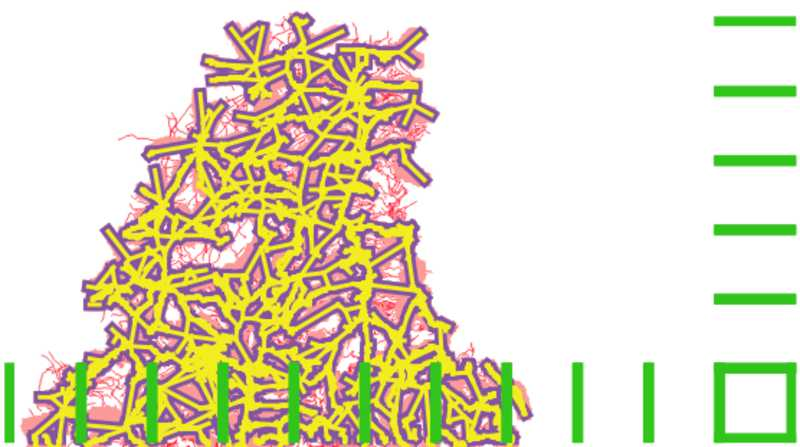
\includegraphics[width=\textheight,angle=90]{Figures/Final/CL-artwork.jpg}
\end{figure}











